
\chapter{Results} 

\label{Chapter5}

%----------------------------------------------------------------------------------------

In this chapter we discuss the results obtained with our model. First, we analyze how the model works in a given (original) resolution, so that we can be confident about its performance. Then, we consider how the accuracy changes with the resolution and within the categories. Finally, we discuss the cost en environment impact around Satellite imagery to analyze the world. 

\section{Transfer Learning on Aerial Imagery}

\section{Man-made Structures Detection at Different Scale}

\begin{figure}[h!]
	\centering
	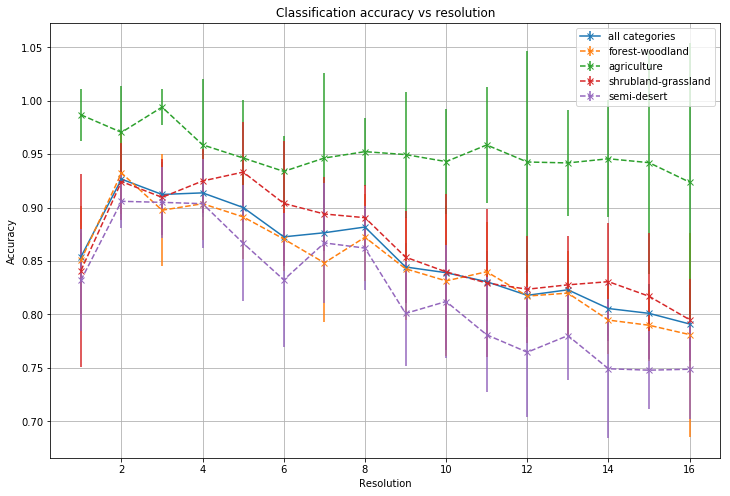
\includegraphics[width=\textwidth]{Figures/results/results_1m_all_categories.png}
	\captionsetup{width=1\linewidth}
	\caption{\textbf{$1m$ dataset}}
	\label{fig:acc_1m_all_cat}
\end{figure}

\begin{figure}[h!]
	\centering
	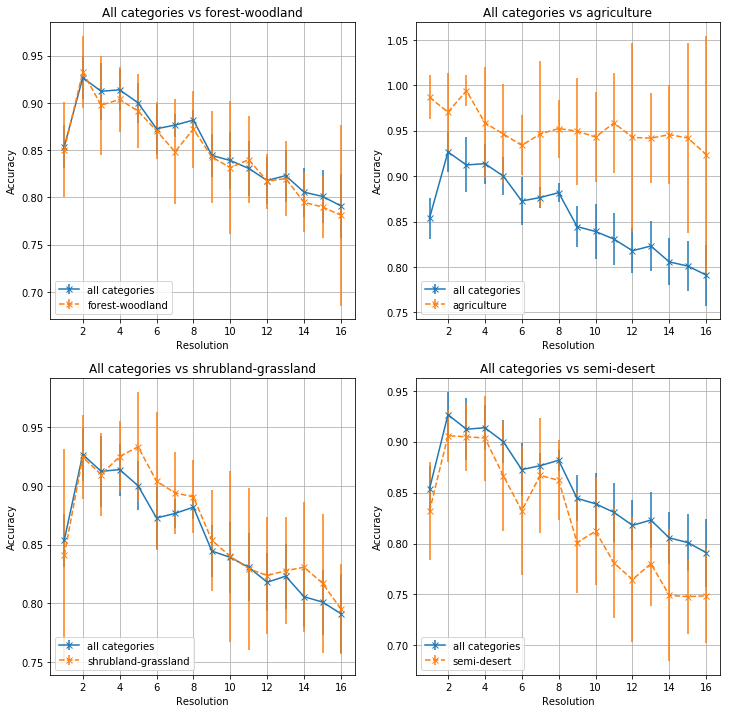
\includegraphics[width=\textwidth]{Figures/results/results_1m_by_category.png}
	\captionsetup{width=1\linewidth}
	\caption{\textbf{$1m$ dataset}}
	\label{fig:acc_1m_byl_cat}
\end{figure}



\section{Cost and Environmental Impact}
It is a very costly business to capture earth imagery data with satellites. Here we discuss both financial cost as well as environmental cost due to carbon footprint required to build and launch a satellite, and to power computational ressources for data processing.
We further study these costs as a function of resolution. However, our estimates are very rough approximations because many are factors involved and large variations occur between them. To give an example, choosing one material over the other might change the cost of manufacturing and launching a satellite by one order of magnitude. It is also completely different to have a satellite for 3 years in space, or to target a lifespan of 20 years. 

Having this in mind, we follow laws from physics to estimate the dependency of the satellite cost on resolution. First, the cost of launching a satellite into the orbit scales linearly with its mass, which is given by the amount of fuel needed. Second, the mass of the satellite scales quadratic with resolution so that overall we obtain a cubic dependency of financial cost on resolution. The latter increase in cost is associated with the optical instruments used. As a reference for the satellite cost we use a Skysat satellite from Planet \parencite{skysat_planet} that has a resolution of about 1m and a value of $\$30$ million. This amount was provided to us by Satellogic and includes construction, launch and maintenance during the satellite's lifespan.

Our final goal is to give an estimation of the expenditure to monitor once the entire surface of the earth (about 149 million km$^2$). To this end, we multiply the satellite cost by the ratio: time needed to scan the earth over the satellite's lifespan. Further, a satellite can map 1 million km$^2$ at 1m resolution in 4.2 days \parencite{satellogic_youtube}. We hence can calculate the satellite cost per km$^2$. With $area/lifespan = 10^6 \times 365/4.2~km^2$ we obtain $cost~satellite~per~km^2 = cost~satellite/area \approx 0.035~\$/km^2$.

\begin{table}[h!]
	\begin{tabular}{l | l | l | l | l}
		description & cost & unit & cost (\$/km$^2$) & cost (\$/pixel) \\
		\hline
		process raw data & & & 0.004 & $4 \times 10^{-9}$ \\
		hot storage  & $72\times 10^{-6}$ & \$/(km$^2$/month) & 0.000864 & $8.64\times10^{-10}$ \\
		cold storage  & $36\times 10^{-6}$ & \$/(km$^2$/month) & 0.000432 & $4.32\times10^{-10}$ \\
		archive storage  & $9\times 10^{-6}$ & \$/(km$^2$/month) & 0.000108 & $1.08\times10^{-10}$ \\
		download data & 8 & \$/Gb & 0.04198 & $4.198  \times 10^{-8}$\\
		serving to final client & 0.09 & \$/Gb & 0.00047232 & $4.7232 \times 10^{-10}$\\
		prediction (AWS) & 0.05 \& $\sim$6 & \$/h \& s/km$^2$ & 0.00145 & $1.45 \times 10^{-9}$\\
	\end{tabular}
	\captionsetup{width=1\linewidth}
	\caption{\textbf{Costs for image data processing.}}
	\label{table:data_costs}	
\end{table}

Another cost intensive block when capturing satellite imagery involves image data processing for which the cost scales quadratic with resolution. For example, an operation that costs 100\$/km$2$ at 1m resolution will cost only 1\$/km$^2$ at 10m resolution. The data processing step consists of multiple parts: transformation of raw data into image pixels, storing data in a hot, cold, and archive storage, downloading data from the satellite, serving it to the final client, and in our case predicting human impact. These costs are summarized for 1m resolution in table \ref{table:data_costs} (provided by Satellogic). Note that we used the conversion factor 0.00524 for an uncompressed image to convert from Gigabytes to km$^2$ and we assume 12 months of data storage. The prediction step represents the prediction of human impact. It is estimated by loading 4 images that each have an area of about $500\times500m^2$, calculating the ResNet activations of the final layer, and predicting the class using the models trained in chapter~\ref{Chapter} in an ensemble fashion. This part amounts to a processing time of 6s for an area of 1km$^2$, which can be converted into costs per km$^2$ assuming 0.05\$/h of AWS EC2 compute~\parencite{aws}.

To finally obtain resolution dependence of the total financial cost we sum the data cost per km$^2$ and the satellite cost per km$^2$ at 1m resolution, and convert to costs per pixel ($\times 10^{-6}$). We then multiply with the number of pixels we need to capture to cover the entire surface of the earth. Here the satellite cost per km$^2$ is a cubic function and the earth surface in pixel is a quadratic function in resolution. We finally obtain the plot shown in Fig.~\ref{fig:costs}. We obtain a cost of about \$15 million dollars at 1m resolution with a very step slope towards better resolutions. At 0.3m resolution the cost is already two orders of magnitued higher than at 1m while for worse resolutions the cost decreases by two orders of magninute when the cost is a factor 10 larger. We conclude that for worse resolutions the data processing cost is the dominating cost whereas for very good resolutions the satellite cost dominates.

\begin{figure}[h!]
	\centering
	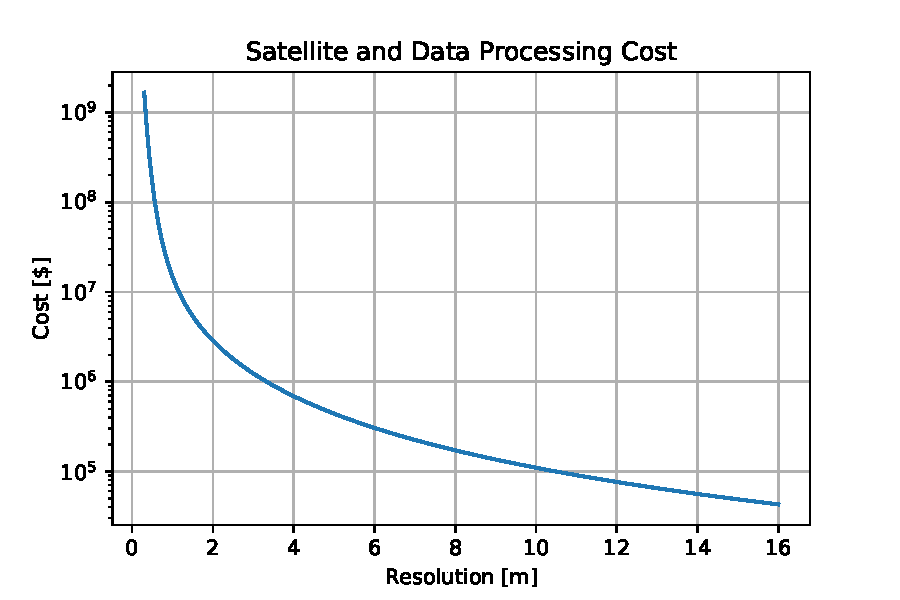
\includegraphics[width=0.75\textwidth]{Figures/costs.pdf}
	\captionsetup{width=1\linewidth}
	\caption{\textbf{Satellite and data processing cost.} The total financial cost to capture images with a satellite and process the data as function of resolution.}
	\label{fig:costs}
\end{figure}

\textcolor{red}{OPTIONAL}
In the remainder of this section we provide a brief discussion about the environmental cost associated to earth observation with satellite's. First, bringing the satellite into orbit is estimated as follows. The satellite needs to reach a certain velocity
\begin{equation}
	v = \sqrt{\frac{G m_e}{R}} \approx 8000 m/s
\end{equation}
parallel to the surface of the earth in order to orbit earth, which can be calculated from the equilibrium between gravitational force $F_g = G m_e m_s / R^2$ and centrifugal force $F_z = m_s v^2/R$. Here $G = 6.67 \times 10^{-11} m^3/(s^2 kg)$ is the gravitational constant, $m_e = 5.9 \times 10^{24} kg$ the mass of the earth, $m_s$ the mass of the satellite, $R = 6371km$ the radius of the earth.
Note that we assume that the distance of the satellite to the surface of the earth is negligible compared to the radius of the earth. The approximate amount of fuel needed to accelerate a satellite to these levels can be calculated using the Tsiolkovsky Rocket Equation \parencite{tsiolkovsky}. We obtain about 12kg of fuel per kg of final satellite weight. With a satellite weight of about 35kg and a factor of 3 to convert Kerosene consumption into CO2 emission \parencite{fuel_to_co2}, we obtain about 1200kg of CO2.
\textcolor{red}{Discuss Carbon footprint of datacenters...}
